\documentclass{article}
\usepackage[utf8]{inputenc}

\usepackage{cite}
\usepackage{amsmath,amssymb,amsfonts}
\usepackage{mathtools}
\usepackage{algorithmic}
\usepackage{graphicx}
\usepackage{textcomp}
\usepackage{xcolor}
\usepackage{braket}
\usepackage{biblatex}
\usepackage{float}
\usepackage{hyperref}

\addbibresource{biblio.bib}

\title{Simulation absorption MALTAB}
\author{Antoine Mingasson}
\date{April 2021}

\begin{document}

\maketitle

\section{Introduction}
Ce document présente le travail que j'ai effectué afin de mettre en place un modèle d'absoprtion des ondes électromagnétiques. Ce modèle est censé reproduire l'effet de l'eau salée sur les ondes électromagnétiques. Il à été codé sur Matlab à partir d'informations trouvés dans la littérature. 

\section{Sources}
Voici les quelques papiers scientifiques qui m'ont permi de créer ce modèle :\\
An Underwater Wireless Sensor Network with Realistic Radio
Frequency Path Loss Model : \href{https://seafile.lirmm.fr/d/fc60846874b44333ae2f/files/?p=\%2FRF\%2Fchannel\%20characterization\%2Fin\%20salted\%20water\%2F2013_508708.pdf}{lien}\\
\\
Path Loss Analysis of RF Waves for Underwater 
Wireless Sensor Networks : \href{https://seafile.lirmm.fr/d/fc60846874b44333ae2f/files/?p=\%2FRF\%2Fchannel\%20characterization\%2Fin\%20salted\%20water\%2F08284460.pdf}{lien}.\\

\section{Formules}
La première étape de la simulation est la détermination de la valeur de permittivité. Cette permittivité est de nature complexe tel que :\\
\[epsilon = epsilon_0*epsilon_R\]\\
avec \(epsilon_0\) la permittivité du vide et \(epsilon_R\) la permittivité relative du milieu.\\
\[epsilon_R = epsilon' - j*epsilon''\]\\
avec \(epsilon'\) la partie réelle de la permittivité relative et \(epsilon''\) la partie complexe de la permittivité relative.\\
Ces deux parties peuvent être définie séparément mais elles peuvent être aussi jointe dans une seule et même formule :\\
\[ epsilon = epsilon_s_w,_\infty\ + (\frac{epsilon_s_w,_0 - epsilon_s_w,_\infty}{1+j*\omega*\theta}) + \frac{\sigma}{\omega * epsilon_0}\]\\
Ou \(epsilon_s_w_\infty\) représente la valeur de permittivité à haute fréquence, qui de fait, est indépendante de la salinité et sera, dans notre cas
fixée à la valeur de 4.9. \(epsilon_s_w_0\) représente la valeur diélectrique statique à basse fréquence. Cette valeur dépend de la salinité du milieu ainsi que de la température, elle est définie tel que :
\[epsilon_s_w,_0(T,S_s_w) = epsilon_s_w,_0(T,0) * a(T,S_s_w) = \] \[(87.134 - 1.949 * 10^{-1}*T - 1.276 * 10^{-2}*T^2 + 2.491 * 10^{-4}*T^3)*\]
\[( 1 + 1.613 * 10^{-5}*T^2 * S_s_w - 3.656 * 10^{-3}*S_s_w + 3.21 * 10^{-5}*S^2_s_w - 4232 * 10^{-7}*S^3_s_w)\]



De plus, on définie aussi \(\theta\) comme :
\[\theta_s_w(T,S_s_w) = \theta_s_w(T,0) * b(T,S_s_w) =\]
\[\frac{1}{2*\pi} * (1.11 * 10^{-10} - 3.824 * 10^{-12} * T + 6.938 * 10^{-14} * T^2 - 5.096 * 10^{-16} * T^3) *\]
\[1 + 2.282 * 10^-2 * T * S_s_w - 7.638 * 10^{-4} * S_s_w - 7.76 * 10^{-6} * S^2_s_w + 1.105 * 10^{-8} * S^3_s_w\]

Une fois la valeur de permittivité calculée, c'est la valeur de conductivité qui doit être déterminée, celle-ci est basé sur la concentration en sel dans le milieu (salinité) ainsi que la température.

\[\sigma = \sigma_0 * \mathrm{e}^{-\phi}\]
avec
\[\sigma_0 = S * ( 0.18252 - 1.4619 * 10^{-3} * S + 2.093 * 10^{-5}*S^2 -  1.282 * 10^{-7} * S^3\]
\[\phi = \Delta * (2.033 * 10^{-2} + 1.266 * 10^{-4} * \Delta + 2.464 * 10^{-6} * \Delta^2) -\] \[S * (1.849 * 10^{-5} - 2.551 * 10^{-7} * \Delta + 2.551 * 10^{-8} * \Delta^2)\]
\[\Delta = 25 - T\]
Dans les résultats et graphes présentés plus tard, c'est la valeur de conductivité mesurée dans l'aquarium qui à été prise au profit de celle calculée par les formules ci-dessus.\\

La constante de propagation est l'étape suivante ; celle-ci représente les changements et effets que va avoir le milieu sur l'onde électromagnétique. Cette constante est calculée de la manière suivante :
\[\gamma = j*\omega*\sqrt{\mu*epsilon - j*\frac{\sigma*\mu}{\omega}} = \alpha + j* \beta\]
La dernière étape est le modèle du Path Loss, ce modèle représente la perte de puissance de l'onde électromagnétiques dans le milieu et lors de changement de milieu soit :
\[PL = L_\alpha,_\epsilon + L_R\]
avec \(L_\alpha,_\epsilon\) représentant les pertes dans le milieu et \(L_R\) qui représente les pertes due à la réflection lors d'un changement de milieu. Dans notre cas, nous allons simplement définir nos pertes dans le milieu comme seules pertes, on a donc :
\(PL = L_\alpha,\epsilon\)\\
ainsi
\[L_\alpha,\epsilon = \Re{(\gamma)} * \frac{20}{ln(10)} * D\]
avec D la distance de propagation.\\



NB : Ces formules et expressions empiriques sont tirées de ce papier \cite{reference_formules}.

\section{Développement du programme}
La mise en place de ce modèle à été assez longue, plusieurs difficultés sont apparues lors de la mise en place de la simulation. Tout d'abord, les formules du modèles étaient parfois différentes selon la source.\\
Après réflexion le papier numéro 1 à été écarté car trop vague sur certains aspects. Je me suis donc penché uniquement sur le 2nd papiers et j'ai finalement réussit à sortir des courbes proches de la littérature. Même si la tendance des courbes de ma simulation reflète bien ce qui est trouvable dans la littérature, il y a quand un facteur d'environ 2 sur la plupart de mes valeurs. Une partie de réponse qui expliquerais cette différence est le fait que les valeurs de température et de salinité de la littérature et ce que j'ai appliqué dans ma simulation ne sont pas parfaitement identiques.

\section{Graphes et résultats de simulation}
Voici quelques graphes comparant les résultats de simulation par ce qu'on peux trouver dans la littérature.

\begin{figure}[H]
    \caption{Absorption de l'eau en fonction de la distance de communication}
    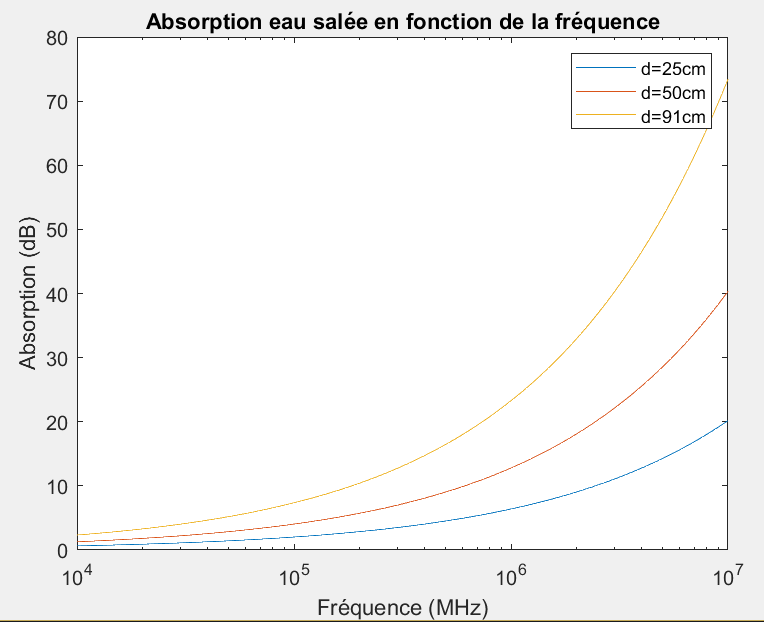
\includegraphics[scale=0.6]{images/distance.PNG}
    \centering
\end{figure}
\begin{figure}[H]
    \caption{Absorption de l'eau salée à plusieurs teneurs en salinité}
    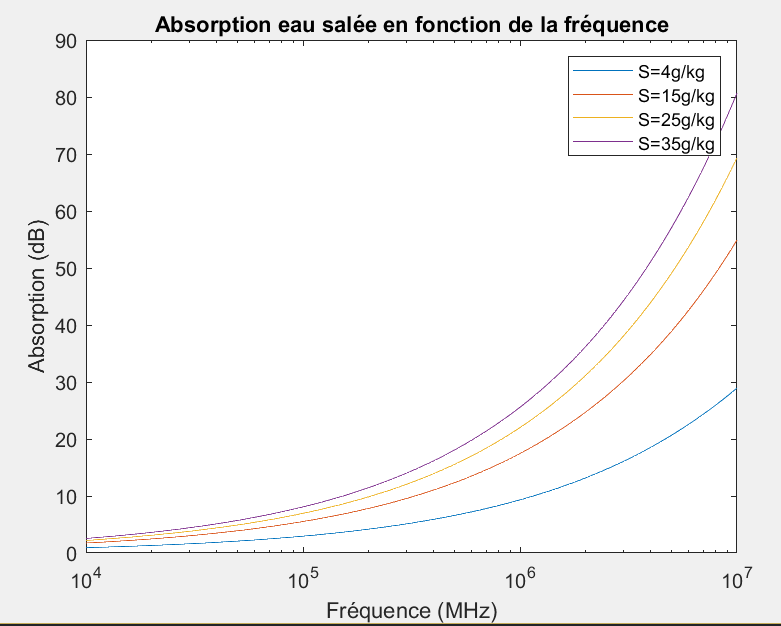
\includegraphics[scale=0.6]{images/sal.PNG}
    \centering
\end{figure}

\begin{figure}[H]
    \caption{Absorption de l'eau salée à plusieurs températures}
    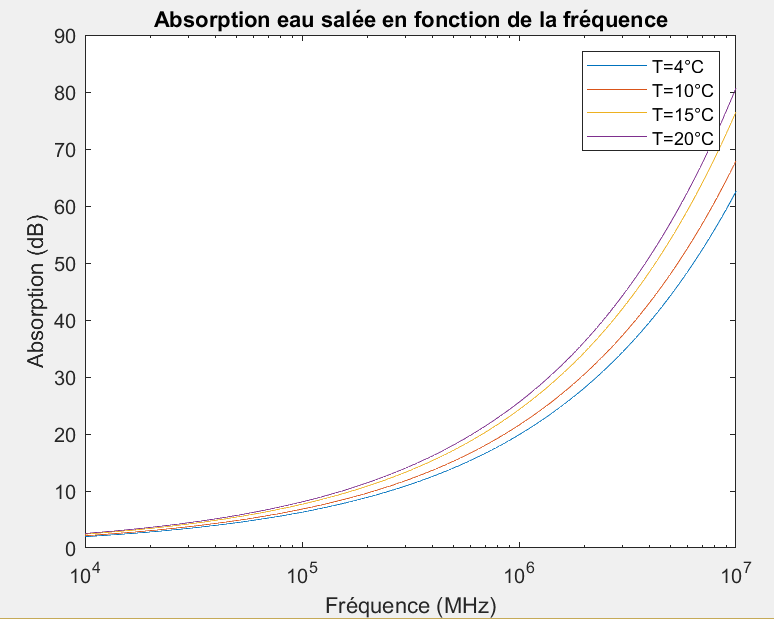
\includegraphics[scale=0.6]{images/temp.PNG}
    \centering
\end{figure}

\begin{figure}[H]
    \caption{Absorption de l'eau salée à plusieurs température (4° et 25°),graphe tiré du papier 1}
    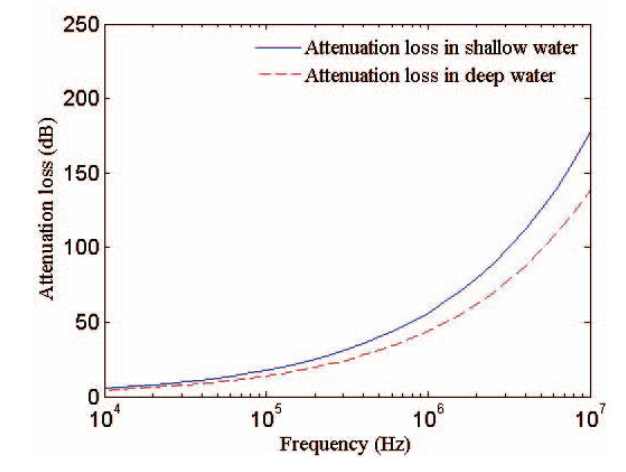
\includegraphics[scale=0.6]{images/papier2.PNG}
    \centering
\end{figure}

\begin{figure}[H]
    \caption{Absorption de l'eau salée à plusieurs fréquences}
    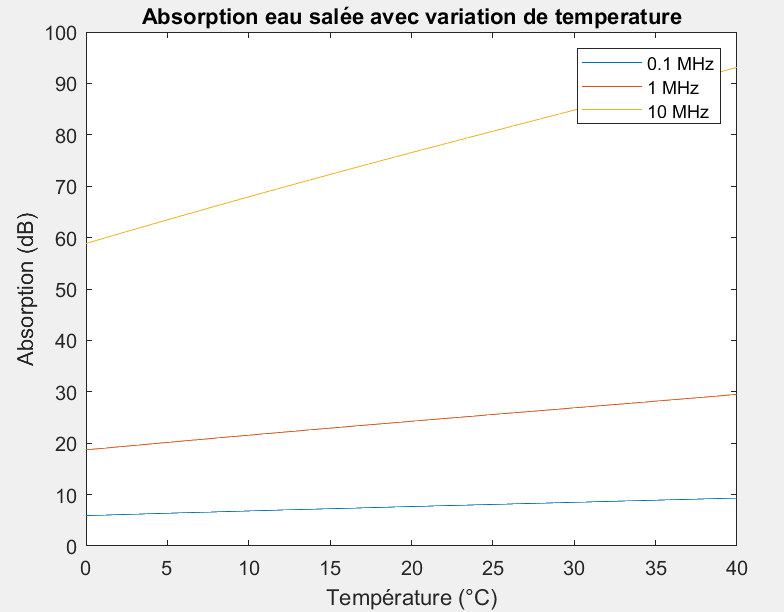
\includegraphics[scale=0.6]{images/freq.PNG}
    \centering
\end{figure}

\begin{figure}[H]
    \caption{Absorption de l'eau salée à plusieurs fréquences,graphe tiré du papier 1}
    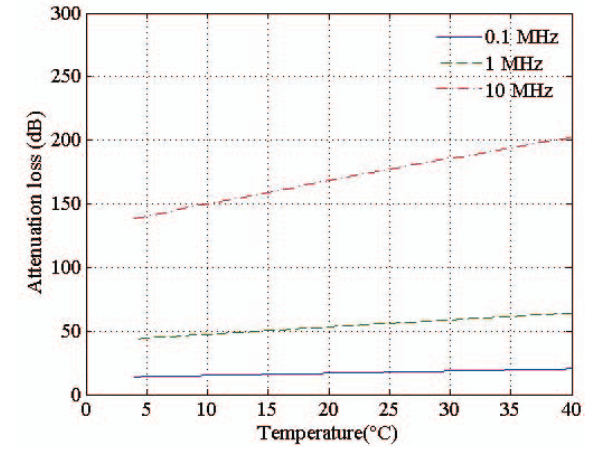
\includegraphics[scale=0.6]{images/papier.PNG}
    \centering
\end{figure}

\printbibliography[title={References}]

\end{document}
